\documentclass[conference]{IEEEtran}
\IEEEoverridecommandlockouts
\usepackage{cite}
\usepackage{amsmath,amssymb,amsfonts}
\usepackage{algorithmic}
\usepackage{graphicx}
\usepackage{hyperref}
\usepackage{textcomp}
\usepackage{xcolor}
\usepackage{listings}
\usepackage{tabularx}
\usepackage{tcolorbox}
\usepackage{array}
\usepackage{fancybox}


\newcommand{\todo}[1]{\textcolor{red}{{\bfseries [[#1]]}}}
\def\BibTeX{{\rm B\kern-.05em{\sc i\kern-.025em b}\kern-.08em
    T\kern-.1667em\lower.7ex\hbox{E}\kern-.125emX}}

\begin{document}

% \title{Do Automated Fault Localization Techniques Work For REST APIs?}
\title{Developing a Comprehensive Taxonomy for REST API Faults: Insights from Real-World Bug Reports}

\author{\IEEEauthorblockN{Aakash Kulkarni}
\IEEEauthorblockA{\textit{School of EECS} \\
\textit{Oregon State University}\\
Corvallis, United States \\
kulkaraa@oregonstate.edu}
\and
\IEEEauthorblockN{Soon Song Cheok}
\IEEEauthorblockA{\textit{School of EECS} \\
\textit{Oregon State University}\\
Corvallis, United States \\
cheoks@oregonstate.edu}
\and
\IEEEauthorblockN{Shreyes Joshi}
\IEEEauthorblockA{\textit{School of EECS} \\
\textit{Oregon State University}\\
Corvallis, United States \\
joshish@oregonstate.edu}
}

\maketitle

\begin{abstract}
    The increasing reliance on REST APIs in modern web applications has highlighted the need for effective fault localization techniques. 
    Existing taxonomies for REST API faults, primarily based on automated test generation tools, focus on error messages and status codes. 
    However, these taxonomies often fail to account for real world issues that can occur in REST APIs, leading to a gap in fault classification. 
    In this study, we analyze real-world bug reports from GitHub to develop a comprehensive taxonomy that encompasses a wider range of fault types. 
    By examining 24 bug reports, we identified 12 distinct categories of faults that are not adequately represented in current taxonomies. 
    Our findings indicate that combining test suite-based taxonomies with bug report-based taxonomies can bridge the gap, providing a more holistic understanding of faults in REST APIs. 
    This new taxonomy aims to enhance fault localization, improve API robustness, and better align with real-world scenarios encountered by developers.
    Alongside this taxonomy, we created a benchmark for evaluating these 24 bugs, which are real world bugs. \\
\end{abstract}


\begin{IEEEkeywords}
Fault Localization, REST APIs, Taxonomies
\end{IEEEkeywords}


% ------------------- Introduction -------------------
\section{Introduction}
\label{sec:introduction}




REST APIs (Representational State Transfer) have become backbone of the modern web and cloud applications. 
They facilitate seamless interactions between client and server through stateless communication, enabling services to be scalable, reliable, and easily integrateable ~\cite{li2016} ~\cite{neumann2018}. 
Basically, REST APIs are a set of rules and standards  defined by OpenAPI ~\cite{ed-douibi2018} used to enable communication between different software applications over the internet. They are built around the use of standard HTTP methods such as GET, POST, PUT, and DELETE to interact with resources, which are any kind of data or service that can be named on a network.
Given their critical role, the effective identification and resolution of faults within REST APIs remain a significant challenge ~\cite{barbir2007}, prompting the need for research on how well the existing taxonomy align with real-world scenarios.

As systems that rely on REST APIs grow in scale and complexity  ~\cite{khare2004} , minor faults can escalate into major disruptions, impacting user experience and business operations. 
So it is important to understand the real-world faults, but there are many faults that can be existing in the context of REST APIs. And we need a detailed taxonomy to cluster these real-world bugs into meaningful categories. So, that we can prioritize and diagnose the critical faults in REST APIs.

Our initial assumption was that the existing taxonomy, developed from automated test generation tools, would align well with real-world bug reports from GitHub. 
To empirically test this assumption, we conducted a study analyzing a set of bug reports from various REST API projects on GitHub. 
Our findings revealed that the existing taxonomy failed to account for real world issues that can occur under successful response codes (e.g., 200 OK). Also, the paper "On the Faults Found in REST APIs by Automated Test Geneation" ~\cite{automatedTestTaxonomy} was limited to the test suite based results and they made a taxonomy based on those results. 
This significant misalignment between the test suite based taxonomy and with real world bugs highlighted the need for a new, comprehensive taxonomy.


Given the shortcomings of the existing taxonomy, our primary objective was to develop a new taxonomy that better represents the faults encountered in real-world scenarios. 
Alongside this taxonomy, we aimed to create a benchmark for evaluating these faults, providing a structured framework for assessing and improving REST API reliability.

And the combining the test-suite based taxonomy and the bug report-based taxonomy, we created a comprehensive taxonomy that encompasses a wider range of faults. 
This new taxonomy aims to provide a more holistic understanding of faults in REST APIs, improving API robustness, and better align with real-world scenarios.


Our Assumptions:

\begin{itemize}
    \item 	\textit{Assumption 1}: We assume that the findings and the new taxonomy can be generalized to other REST API projects beyond the ones specifically analyzed in this study.
    \item   \textit{Assumption 2}: 	We assume that the new taxonomy will provide better diagnostic capability for developers, allowing them to identify, categorize, and prioritize faults more effectively.
\end{itemize}



The motivation for this research stems from the critical need to address the gap between theoretical fault models derived from automated test generation tools and the practical issues encountered in real-world REST API applications. 
Existing taxonomies primarily focus on certain types of errors, such as 500-based errors, and often fail to account for faults that occur under successful response codes like 200 OK. 
This misalignment limits the ability of developers to effectively diagnose, categorize, and prioritize faults. By creating a new, comprehensive taxonomy based on real-world bug reports, we aim to provide a more accurate and practical framework for understanding REST API faults. 
This taxonomy will enhance  fault understanding process, improve system reliability, and better support developers in maintaining robust and resilient REST API-based systems.

To guide our investigation and address the identified gaps, we formulated the following research questions:
\begin{enumerate}
    \item \textbf{RQ1:} What categories of faults are most prevalent in real-world REST API bug reports?
    \item 
\end{enumerate}


For the evaluation dataset, we will manually select the issues from the GitHub services and their fixes from REST API projects that utilize Spring Boot or Jersey frameworks. These GitHub services are used in the paper  \textit{Generating REST API Specifications through Static Analysis} by Manish et al ~\cite{ManishRestServices}
This dataset will encompass various categories of faults identified in REST APIs. By analyzing repositories and commit histories, we will extract specific instances where bugs have been documented and subsequently fixed. 


Our analysis of bug reports led us to create a benchmark of 24 bugs which were classified with a taxonomy based on bug reports.

In the following sections we will describe our methodology and results.

% This research is motivated by the need to evaluate how well current fault localization techniques perform in the unique context of REST APIs. 
% The goal is to determine if these techniques can indeed be applied effectively to REST APIs and, if so, to explore which types of faults are more amenable to being localized. 
% This understanding could potentially allow developers to more efficiently diagnose and address issues, thereby enhancing the stability and performance of REST API-based systems.

% Fault localization is a well-established area of research within software engineering, traditionally concentrated on more conventional software systems. 
% REST APIs, however, present distinct challenges that complicate fault localization due to their composition and operational dynamics. 
% Additionally, the architecture of REST APIs often involves diverse artifacts that are not source code, such as configuration files, API specifications, and database schemas.

% The primary objective of this research is to evaluate the effectiveness of existing fault localization techniques within the unique context of REST APIs, which feature a mix of code and non-code artifacts. 
% This study will systematically apply established fault localization methods like BLUES ~\cite{ManishBluesFaultLocalization} and LLMAO ~\cite{LLMAOFaultLocalization} to a dataset of REST API faults. 
% This dataset will be meticulously developed to represent a wide range of faults typical in REST APIs and classified according to an existing comprehensive taxonomy derived from previous research.

% This approach will enable us to assess the applicability of these fault localization techniques to REST APIs by determining how effectively they can identify and localize different types of faults. 
% The analysis will provide insights into whether traditional fault localization methods are suited to the complexities of REST APIs, especially considering their unique structural and functional characteristics.


% % ----------------- Assumptions -----------------
% Our assumptions:
% \begin{itemize}
%     \item \textit{Assumption 1:} Assume that the dataset of REST API faults would fit in the taxonomy that we have developed. 
%     \item \textit{Assumption 2:} Assume that the selected fault localization techniques are suitable for application to REST APIs, despite their original design for conventional software systems. This includes the assumption that these techniques can handle the unique challenges posed by REST APIs, such as dealing with non-code artifacts.
% \end{itemize}


% % ------------------- Research Questions -------------------
% The primary research questions are formulated as follows:
% \begin{itemize}
%     \item \textbf{RQ1:} What categories of faults are most effectively localized by current techniques?
%     \item \textbf{RQ2:} Which fault localization technique is highly effective in the context of REST APIs?
% \end{itemize}

% For the evaluation dataset, we will manually select the issues from the GitHub services and their fixes from REST API projects that utilize Spring Boot or Jersey frameworks. These GitHub services are used in the paper  \textit{Generating REST API Specifications through Static Analysis} by Manish et al ~\cite{ManishRestServices}
% This dataset will encompass various categories of faults identified in REST APIs. By analyzing repositories and commit histories, we will extract specific instances where bugs have been documented and subsequently fixed. 
% The categorization of these faults will be categorized with an established taxonomy of API faults ~\cite{automatedTestTaxonomy} , ensuring that each bug is classified according to its nature and impact. This rigorous dataset compilation aims to provide a comprehensive basis for testing fault localization techniques within a controlled, relevant environment.

% For evaluation of fault localization techniques using the dataset derived from REST APIs employing Spring Boot and Jersey frameworks will be measured by Top-k accuracy, and EXAM score.
% These metrics will collectively provide a thorough assessment of each fault localization technique's ability to detect and accurately categorize faults in REST APIs, contributing to a detailed understanding of their practical utility and areas for improvement.


% ------------------- Background and Motivation -------------------
\section{Background and Motivation}
\label{sec:background-and-motivation}

\subsection{Importance of REST APIs}
REST APIs (Representational State Transfer APIs) are central to modern web and cloud applications, serving as critical conduits for data exchange and system integration. 
They leverage standard HTTP methods like GET, POST, PUT, and DELETE to interact with networked resources, making them integral to the architecture of distributed systems. 
The scalability, reliability, and ease of integration provided by REST APIs facilitate seamless interactions between clients and servers, thereby enhancing the performance and flexibility of complex software ecosystems. 
Their widespread adoption underscores their importance in today's technology landscape, where rapid communication and data accessibility are paramount.

% \subsection{Challenges of Fault Localization in REST APIs}
% While REST APIs have simplified the development and management of modern applications, they introduce specific challenges that complicate fault localization.
% The architecture often involves non-code artifacts such as API specifications, configuration files, and database schemas, which are not traditionally addresses by fault localization techniques developed for code-centric applications. 

\subsection{Gaps in Current Research}
% Fault localization is a well-established research area within software engineering, focusing primarily on identifying the locations of faults in conventional software systems to reduce debugging time and enhance system reliability.
%  However, 
The unique operational dynamics and architectural complexities of REST APIs pose new challenges that are not fully addressed by existing to create a comprehensive taxonomy.
Previous studies have developed fault taxonomies for REST APIs which are helpful only in categorizing based on the failed test cases.
% if the FL techniques can localize faults to understand what categories of faults can be localized.




% \subsection{Need for Targeted Research on Fault Localization in REST APIs}
% This research is motivated by the critical need to evaluate and understand the performance of existing fault localization techniques within the REST API context. 
% By determining how effectively these techniques can identify and localize faults in REST APIs, developers can gain valuable insights that could lead to quicker and more accurate fault diagnosis. This is particularly important as even minor faults can escalate into major disruptions in REST API-dependent systems, affecting user experience and operational efficiency. Addressing this gap will not only contribute to the field by enhancing the robustness and reliability of REST APIs but also by supporting the development of more sophisticated tools and methodologies tailored to the needs of modern software architectures.

% \subsection{Research Objectives}
% The primary objective of this research is to systematically assess the applicability of established fault localization techniques—namely 
% BLUES and LLMAO to a curated dataset of REST API faults. 
% This dataset will be developed to encompass a broad spectrum of typical faults in REST APIs and will be classified according to an existing comprehensive taxonomy. 
% The insights gained from this study are expected to reveal whether traditional fault localization methods are suitable for the complex environments of REST APIs and may guide future efforts in refining these techniques or developing new approaches specifically designed for REST API ecosystems.

\begin{figure*}[t] 
    \centering
    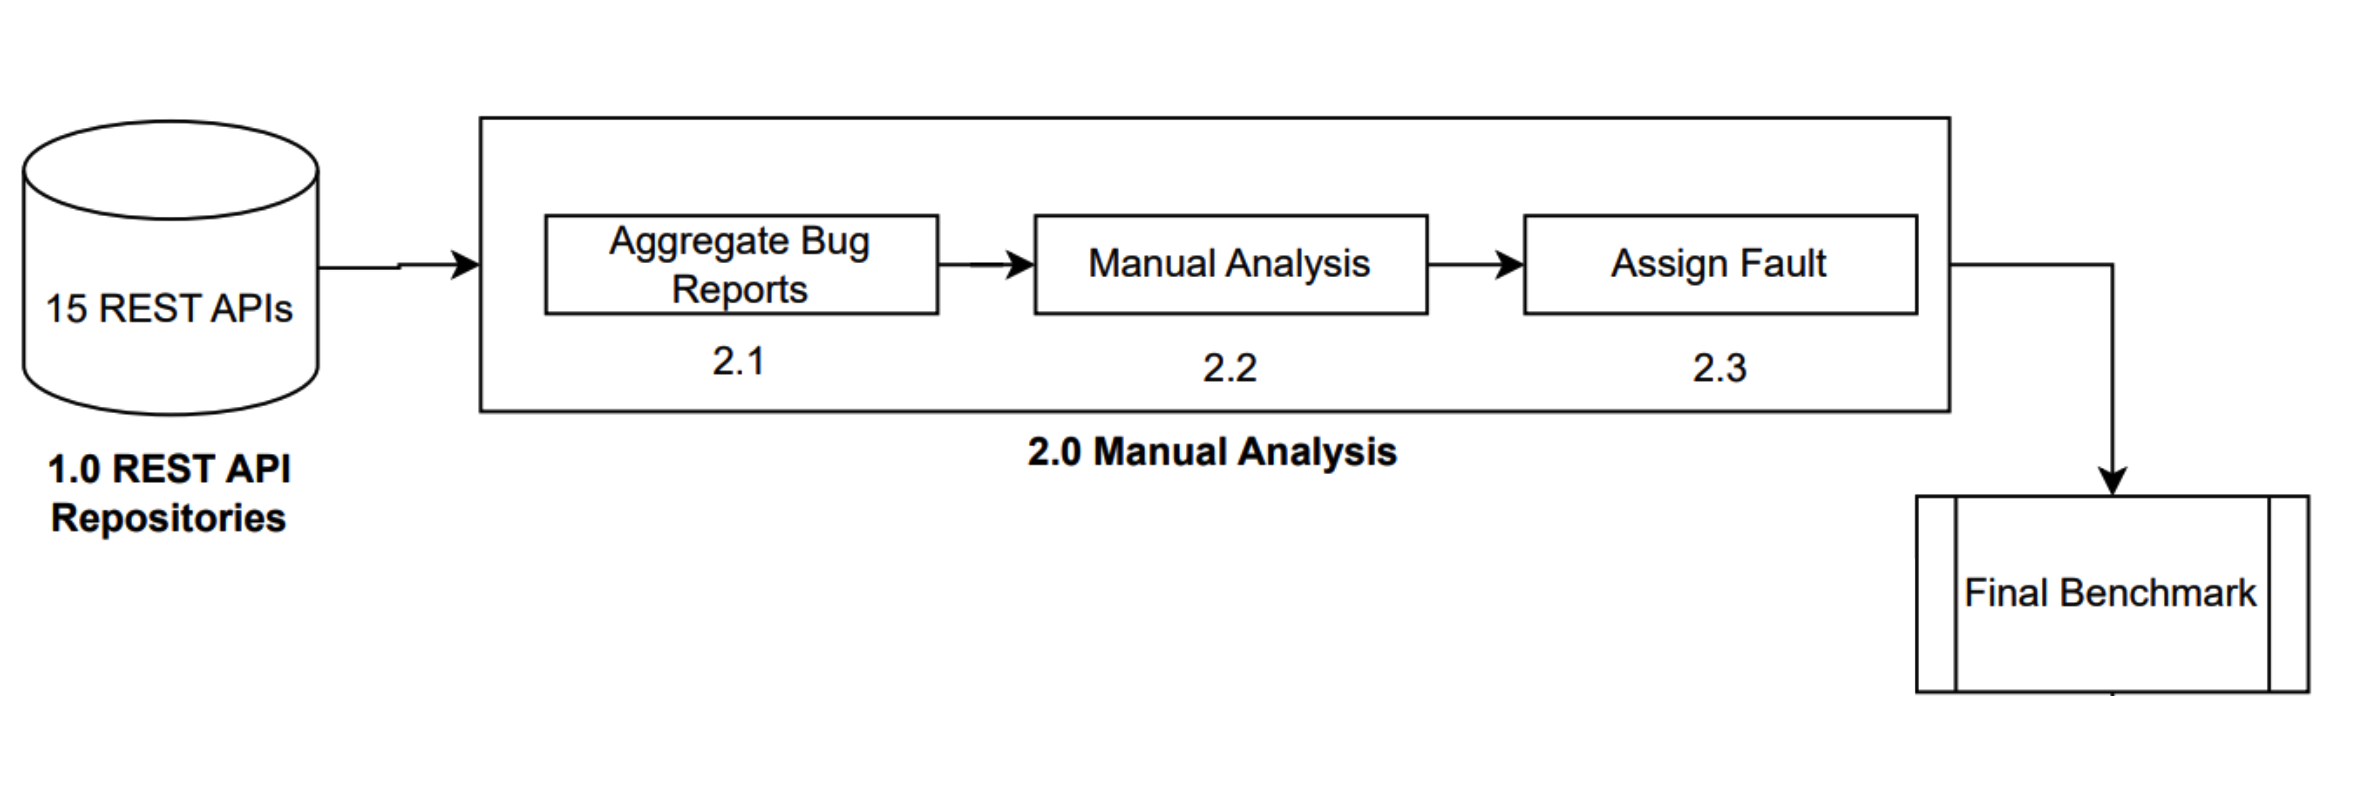
\includegraphics[width=1.0\textwidth]{FaultTaxonomyFlow.png}
    \caption{Approach Overview}
    \label{fig:widefigure}
  \end{figure*}



%   ------------- Related Work -------------
\section{Related Work}
\label{sec:relatedwork}

\begin{figure*}[t] 
    \centering
    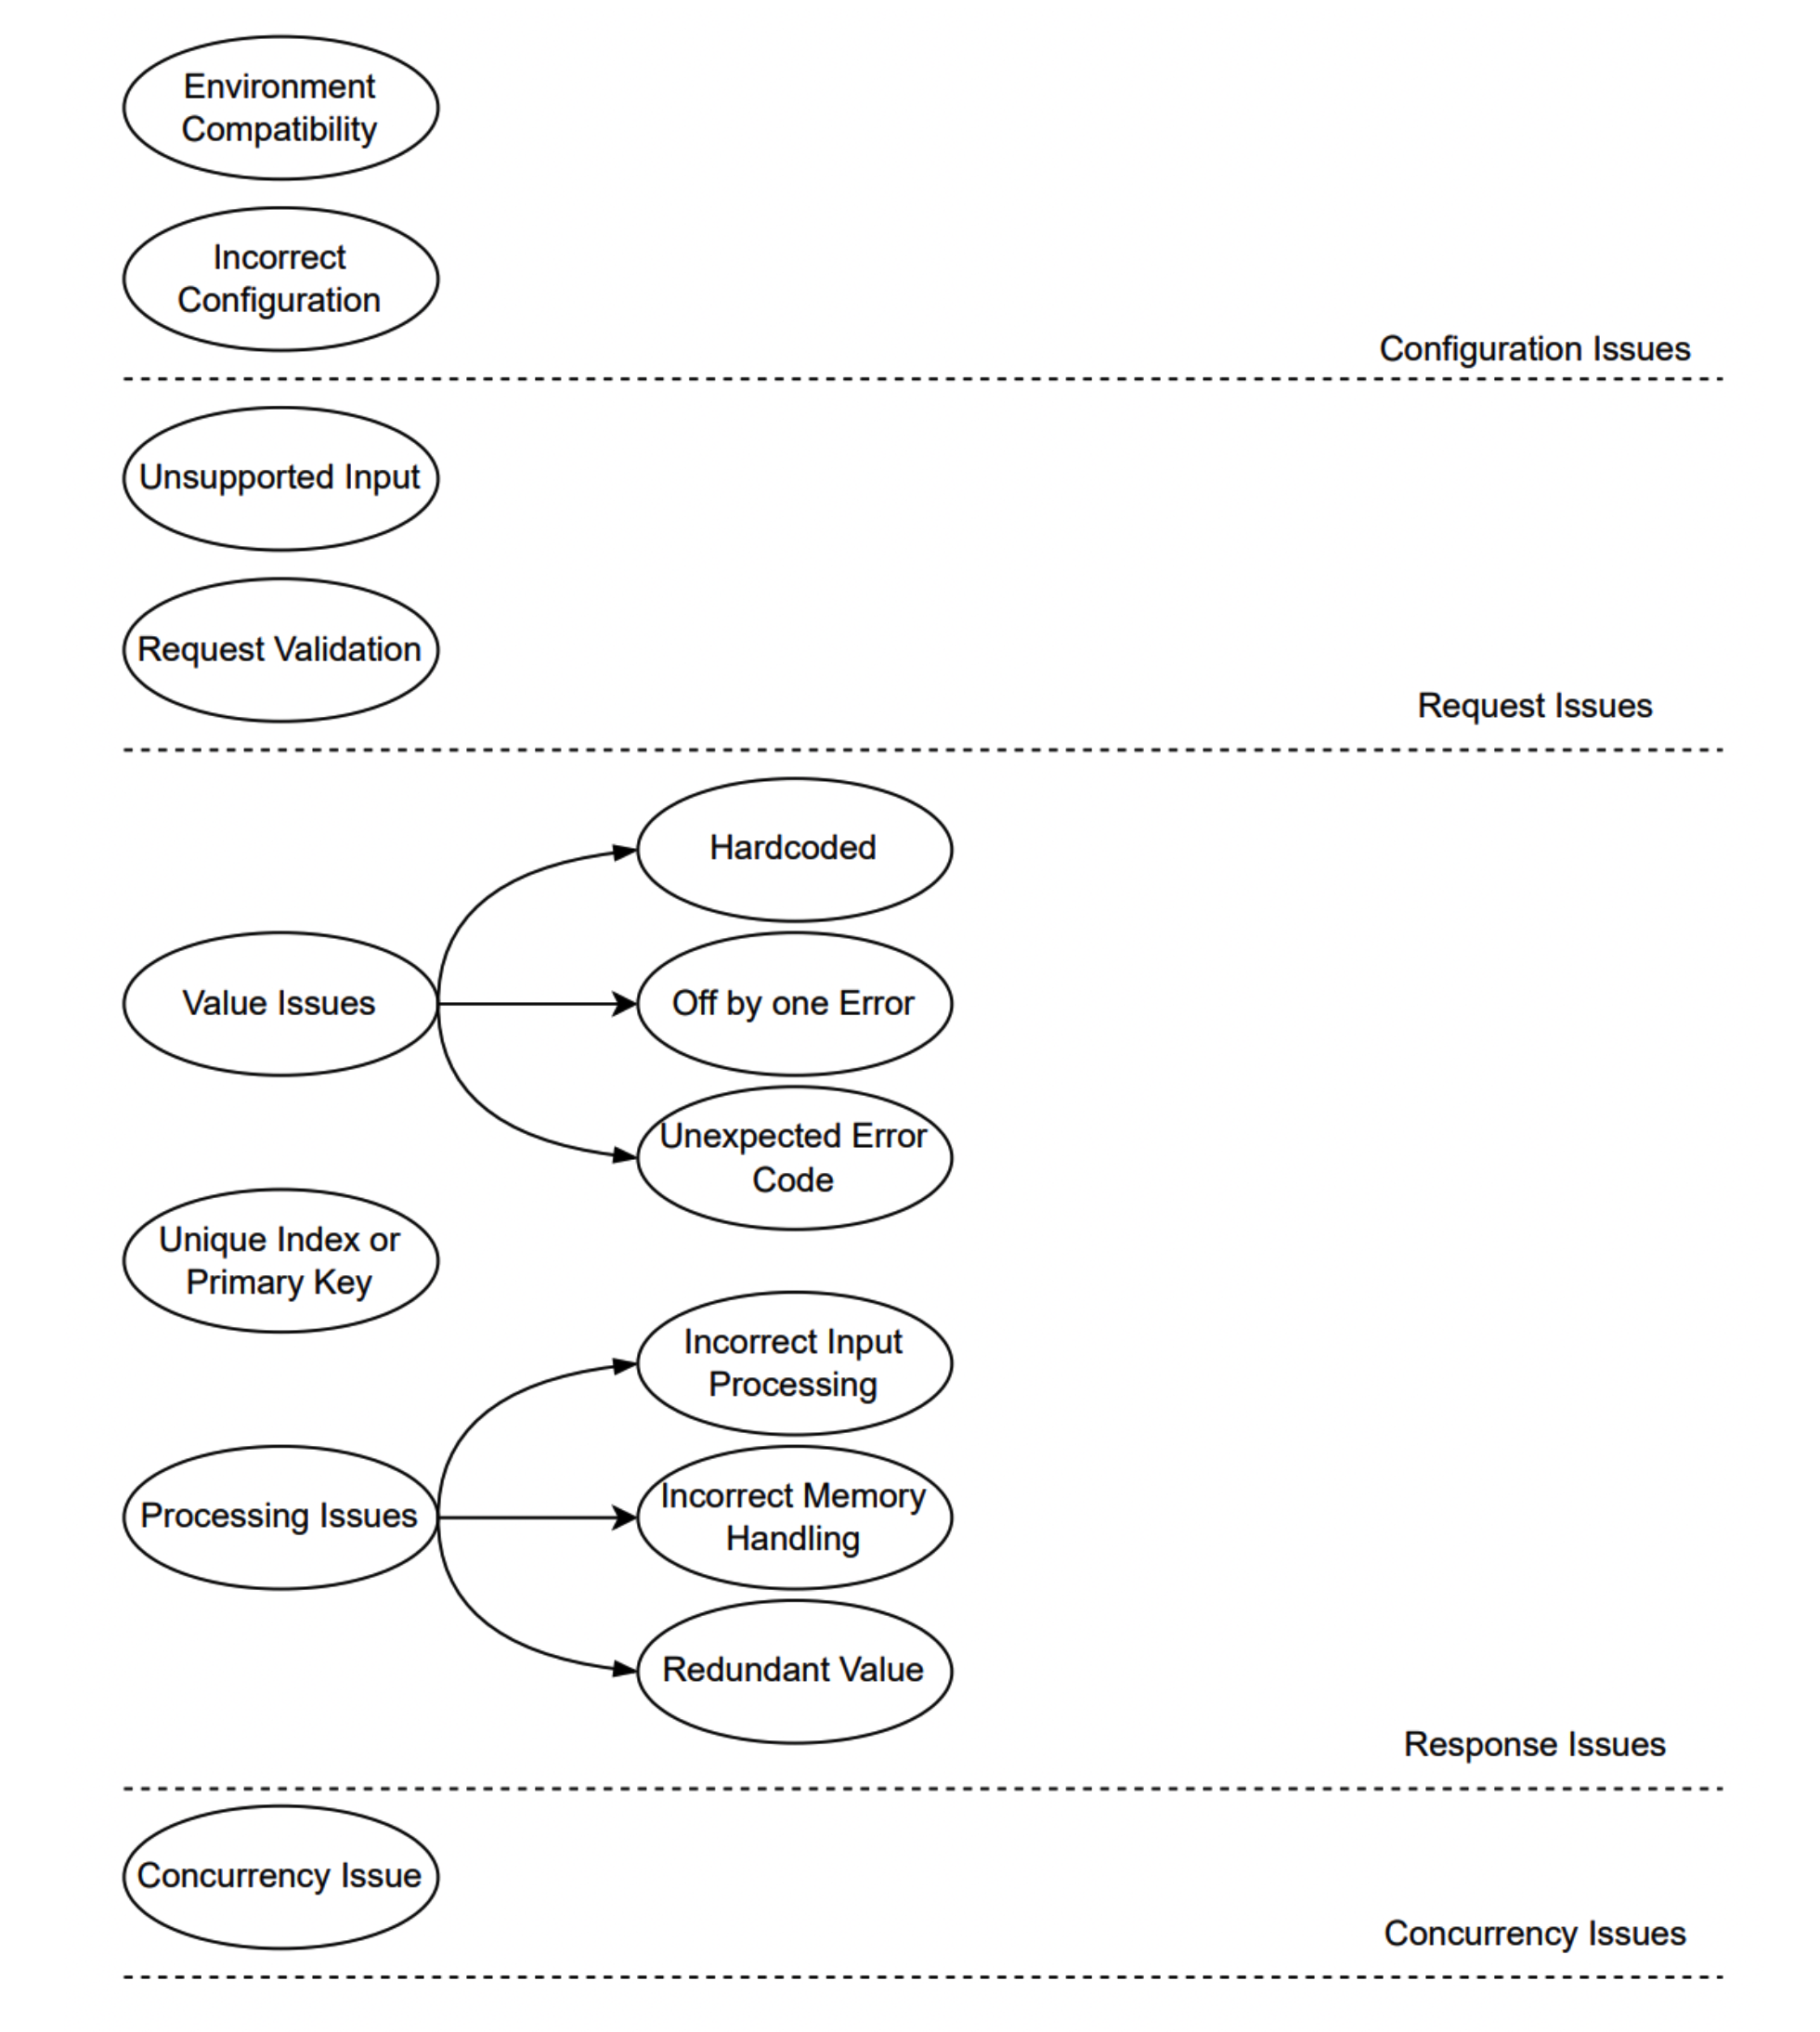
\includegraphics[width=0.8\textwidth]{TaxonomyDeveloped.png}
    \caption{Developed Taxonomy}
    \label{fig:TaxonomyDeveloped}
  \end{figure*}


% Fault localization techniques have long been an integral part of software maintenance, aiding developers by pinpointing the origins of failures within software systems. 
% A variety of approaches have been explored ~\cite{Wong2023_Software_Fault_localization}, including Information Retrieval (IR) based methods, Spectrum-Based Fault Localization (SFL), and more comprehensive software engineering tools.


% BLUES (Bug Localization Using Error Messages and Stack Traces) is a fault localization technique designed to enhance the accuracy and efficiency of identifying the sources of bugs in software systems. Developed by  Manish et al ~\cite{ManishBluesFaultLocalization} , BLUES leverages bug reports to pinpoint potential fault locations within the codebase.

% LLMAO is a fault localization technique that leverages large language models (LLMs) to identify and rank potential fault locations within software systems. Developed to utilize the capabilities of advanced LLMs, LLMAO provides a novel approach to fault localization by analyzing code changes and utilizing commit history.

% And there is a
% The paper about the fault taxonomy, The paper titled “On the Faults Found in REST APIs by Automated Test Generation” \cite{automatedTestTaxonomy} investigates the types of faults that can be uncovered through the use of automated test generation tools. This research provides a taxonomy of faults specifically found in REST APIs by analyzing the failures encountered during automated testing.
% This is the only paper we found which was trying to create a taxonomy of faults for the REST API applications, as it was limited to the test suite based results and they made a taxonomy based on those results. Also, the classification they have done heavily manual and there is not automated classification method that exists right now which can address the issue of clustering the faults into categories


The paper titled “On the Faults Found in REST APIs by Automated Test Generation” \cite{automatedTestTaxonomy} investigates the types of faults that can be uncovered through the use of automated test generation tools. This research provides a taxonomy of faults specifically found in REST APIs by analyzing the failures encountered during automated testing. The study meticulously categorizes various fault types based on the error messages and behavior observed when automated test cases are executed against REST API endpoints.

This is the only paper we found that attempts to create a comprehensive taxonomy of faults for REST API applications. However, its scope is limited to faults identified through test suites. The taxonomy developed in this research is based on the results of these automated tests, which primarily detect faults resulting in error status codes, such as 500 Internal Server Errors. Consequently, this taxonomy may not capture the full range of faults that occur in real-world scenarios, particularly those that manifest under successful response codes.

Furthermore, the classification process in this paper is heavily manual, involving significant human effort to categorize the faults based on their characteristics. Currently, there is no automated classification method that can effectively cluster these faults into meaningful categories. This reliance on manual classification poses challenges in scalability and consistency, as the subjective nature of human judgment can lead to variations in fault categorization.

Overall, while this research provides valuable insights and a foundational taxonomy for REST API faults, its limitations highlight the need for a more comprehensive and automated approach to fault classification. 
% Our research aims to address these gaps by developing a new taxonomy based on real-world bug reports and creating a benchmark for evaluating faults, which will facilitate more accurate and efficient fault localization in REST API systems.

% Debugging in IDEs, particularly using tools like Visual Studio Code for web applications, illustrates the practical aspects of fault localization in real-world scenarios ~\cite{DebuggingCode}. The capabilities of IDEs to facilitate debugging through breakpoints and variable inspections are directly relevant to the challenges faced in REST API development, where faults may not only arise from code but also from API configurations and interactions.




%   ------------- Approach ------------
\section{Approach}
\label{sec:approach}

\subsection{Dataset Creation and Preparation}

% To effectively assess the applicability of fault localization techniques to REST APIs.
In our research, we utilize a set of REST API services previously employed in the study "Generating REST API Specifications through Static Analysis" by Manish et al ~\cite{ManishRestServices}. These services are chosen due to their diverse characteristics and well-documented configurations, making them suitable subjects for evaluating fault localization techniques. 
% The faults from these services will be categorized based on a previously established taxonomy of REST API faults, ensuring that each fault type is adequately represented. 

We are three graduate students with knowledge on REST API, we have selected the issues on GitHub Repositories, and we have the read the bug reports of the issues and saw what were the changes made and assigned it a fault type. We all have gone through all the services and then we together consolidated into one single list where we found 24 Faults which we can test using the Fault Localization Techniques. 
There were almost 50 bugs we had discussed, and we are confident about these 24 bugs in our dataset. And the others are pruned for now because we are not confident enough about those.

% \subsection{Selection of Fault Localization Techniques}

% The study will focus on two primary fault localization techniques that have shown promise in traditional software contexts but whose effectiveness in REST APIs remains underexplored:
% \begin{enumerate}
%     \item \textbf{BLUES:} ~\cite{ManishBluesFaultLocalization} BLUES is developed by a group of researchers Manish et al which takes Bug report as input and generates the suspicious ranked list of faulty code.
%     \item \textbf{LLMAO:} ~\cite{LLMAOFaultLocalization} LLMAO is developed by a group of researchers Aidan et al, where LLMAO is first LLM (Large Language Model) based for fault localization and which takes no inputs. But it finds the difference between two commits to see where the bug was introduced and creates a ranked list of faulty code. 
% \end{enumerate}

% Both the Fault Localization Techniques are known for their effective finding of the faulty code. And also both the techniques are new.

\subsection{Integration with REST API Characteristics}
Given the unique challenges posed by REST APIs, such as stateless operations and the presence of non-code artifacts (e.g., configuration files and API specifications), our approach will also consider these elements:
\begin{itemize}
    \item \textbf{Non-Code Artifacts}: Special attention will be given to faults that may originate from or affect non-code artifacts. 
\end{itemize}

% \begin{figure*}[t]
%     \caption{Issue Types}
%     \label{fig:issueTypes}
%     \begin{tabular}{|m{3cm}|m{3 cm}|m{5cm}|m{5cm}|}
%     \hline
%     \textbf{Concurrency Issues} & \textbf{Configuration Issues} & \textbf{Implementation Issues} & \textbf{Verification and Validation Issues} \\
%     \hline
%     Concurrency Issue & Environment Incompatibility & \textbf{Coding Issues:} & Request Verification \\
%      &  & Hardcoded &  \\
%      & Incorrect Configuration & Off by one Error & Unexpected Error Code \\
%      &  & Unsupported Code &  \\
%     \hline
%      &  & \textbf{Processing Issues:} &  \\
%      &  & Incorrect Input Processing &  \\
%      &  & Incorrect Memory Handling &  \\
%      &  & Redundant Value &  \\
%     \hline
%      &  & \textbf{Indexing Issues:} &  \\
%      &  & Unique Index or Primary Key &  \\
%     \hline
%     \end{tabular}
% \end{figure*}




%   ------------- Evaluation ------------
\section{Evaluation}
\label{sec:evaluation}



%   ------------- Dataset ------------
\subsection{Dataset}
\label{sec:dataset}

To conduct this research, a dataset is required for evaluation. The dataset contains REST API faults, their sources, and other relevant information necessary like Bug Reports to evaluate FL techniques.

The dataset we started with had  GitHub APIs from 15 different REST API repositories from the services were management-api-for-apache-cassandra, catwatch, cwa-verification-server, digdag, enviroCar-server, features-service,
gravitee-api-management, kafka-rest, ocvn, ohsome-api, proxyprint-kitchen, quartz-manager, restcountries, senzing-api-server, and Ur-Codebin-API.
The  process of filtering out issues not marked as 'bugs' and 'closed,' leaving only the set of issues that have been fixed details ~\ref{tab:repositories}. Issues involving code changes are collected and then further filtered through manual analysis to select those applicable to this research. These services provide us services with bug information we need to create a benchmark on REST API faults.

\begin{table}
    \centering
    \caption{List of Repositories}
    \label{tab:repositories}
    \begin{tabular}{|c|l|c|}
    \hline
        \hline
        \textbf{No.} & \textbf{Repository Name} & \textbf{\# of Faults} \\ \hline
        1 & management-api-for-apache-cassandra & 2 \\ \hline
        2 & cwa-verification-server &  7 \\ \hline
        3 & digdag & 2 \\ \hline
        4 & ohsome-api & 10 \\ \hline
        5 & kafka-rest & 3 \\ \hline
    \end{tabular}
\end{table}
    

Our initial assumption that the existing taxonomy would be sufficient proved incorrect, prompting us to develop our own taxonomy. 
When we encountered issues not covered by the existing taxonomy, we created new categories. Out of the 24 bugs analyzed, only 2 could be classified using the existing taxonomy. 
However, even for these, the alignment between the bug reports and the fault type definitions was not ideal.

\subsection{The Taxonomy}
\label{sec:newtaxonomy}

Based on our analysis of the 24 bug reports from various REST API projects, we developed a comprehensive taxonomy ~\ref{fig:TaxonomyDeveloped} that encompasses a broader range of fault types not adequately captured by existing taxonomies. This new taxonomy is categorized into major fault categories, each containing specific fault types.

Major Categories and Fault Types

\subsection{Major Categories and Fault Types}

\begin{enumerate}
    \item \textbf{Concurrency Issues}
    \begin{itemize}
        \item \textbf{Concurrency Issue:} This fault refers to a scenario known as a race condition in concurrent programming, where two functions are intended to execute sequentially but run simultaneously instead. This can result in one function depending on the output of the other function before it has completed, leading to erroneous outcomes or failures.
    \end{itemize}
    
    \item \textbf{Configuration Issues}
    \begin{itemize}
        \item \textbf{Environment Incompatibility:} These are the kind of errors which arise due to the environments such as Operating System, Hardware Environment, or Network Environment, where the code written for one environment doesn't translate to another environment.
        \item \textbf{Incorrect Configuration:} This fault refers to errors or mistakes in the setup or configuration of a system, software, or application. Misconfiguration can lead to unexpected behavior, errors, or issues.
    \end{itemize}

    \item \textbf{Implementation Issues}
    \begin{itemize}
        \item \textbf{Coding Issues:}
        \begin{itemize}
            \item \textbf{Hard-coded:} This fault type occurs when a value is invalid due to being Hard-Coded within the software.
            \item \textbf{Off by one Error:} An off-by-one error refers to a programming mistake where the application incorrectly processes or manipulates data, resulting in either accessing one more or one less element than intended, leading to unintended behavior or functional errors in the web application.
            \item \textbf{Unsupported Input:} This issue occurs when the documented functionality or parameters are not implemented or supported in the actual codebase or system. This discrepancy can lead to unexpected behaviors, errors, or limitations when utilizing the software based on the documented specifications.
        \end{itemize}

        \item \textbf{Processing Issues:}
        \begin{itemize}
            \item \textbf{Incorrect Input Processing:} Incorrect input processing in web applications refers to the improper handling of user inputs, leading to issues such as errors in API responses, unexpected behavior, and inconsistencies in the way data is processed and displayed. This can result in inaccuracies, unexpected outcomes, and functionality failures within the web application.
            \item \textbf{Incorrect Memory Handling:} Incorrect memory handling involves inadequate or absent measures to limit or manage memory usage within a system, potentially leading to issues like memory exhaustion, performance degradation, or system instability.
            \item \textbf{Redundant Value:} This fault type refers to an unnecessary or duplicated data point or condition within a system, schema, or dataset. It indicates an extra check or condition that adds complexity without providing any additional benefit in terms of data validation or processing logic.
        \end{itemize}

        \item \textbf{Indexing Issues:}
        \begin{itemize}
            \item \textbf{Unique Index or Primary Key:} This fault arises when an identifier, such as an ID or key, is shared by multiple entities or records. This lack of uniqueness can result in data inconsistency, referencing errors, and challenges in accurately identifying or distinguishing individual entities within the system.
        \end{itemize}
    \end{itemize}

    \item \textbf{Verification and Validation Issues}
    \begin{itemize}
        \item \textbf{Request Verification:} This refers to the process of confirming the validity and authorization of incoming requests made to a system or application. This involves checking user permissions, ensuring proper authentication, and validating the data provided in the requests to prevent unauthorized access, maintain security, and uphold data integrity within the system.
        \item \textbf{Unexpected Error Code:} This occurs when an error code is generated in response to a specific condition that deviates from the expected or standard error code for that situation.
    \end{itemize}
\end{enumerate}


%   ------------- Metrics ------------
% \subsection{Metrics}
% \label{sec:metrics}

% There are several metrics that can be used to evaluate how effective FL techniques are at localizing REST API faults. In this research, two primary metrics to consider are \textbf{Top-k Accuracy}, and \textbf{EXAM}.

% \textbf{Top-k Accuracy:} This metric measures the percentage of actual faulty statements found within the top k position of the ranking generated by an FL technique. The ranking positions are based on how likely each statement is considered faulty according to the fault localization algorithm. This metric is useful for evaluating how effective FL techniques are at localizing faults. In this research, several values of k are used to measure the FL technique's performance, such as top-1, top-5, and top-10.
% \\
% This metric measures the percentage of times the actual faulty statements are within the top $k$ positions of a ranked list produced by the fault localization technique. Mathematically, it is expressed as:
%     \[
%         \text{Top-k} = \frac{\text{ \#faults found in top } k \text{ positions}}{\text{Top k positions }} \times 100\%
%     \]
%     This metric evaluates the effectiveness of fault localization techniques by their ability to rank the actual faulty statements highly on the list.
%     \\
%     \textbf{EXAM score:}  This metric is defined as the percentage of the total statements a developer needs to examine before finding the fault statement. A low EXAM score indicates that the fault localization technique was able to rank faulty statements highly, reducing the amount of code that needs to be inspected. This reflects an effective fault localization technique that quickly directs developers to the most likely faulty areas. 
%     However, the EXAM score does not account for multiple faults, limiting its ability to measure the effectiveness of an FL technique for multiple faults.
%     The EXAM score is calculated as the percentage of the code that must be examined until the first occurrence of a fault is encountered. It is defined as:
%     \\
%     \[
%         \text{EXAM Score} = \frac{\text{Number of statements before fault}}{\text{Total number of ranked statements}} \times 100\%
%     \]
%     A lower EXAM score indicates a more effective fault localization technique, as it suggests that fewer statements need to be inspected before finding the fault. This metric is particularly useful for assessing the efficiency of a technique in directing developers quickly to the likely fault locations.
%     \\ \\
%     \textbf{Precision}: This metric measures the fraction of actually faulty statements out of the total reported faulty statements. It provides a measurement indicating how well an FL technique can localize faults. However, it doesn't capture an FL technique's capability to localize all faults.
%     \\

% The metrics are effective measures of FL technique performance. They will be used to measure how well FL techniques can localize REST API faults.


%   ------------- Experiment Procedure ------------
% \subsection{Experiment Procedure}
% \label{sec:experiment-procedure}

% The objective of our experiments is to systematically evaluate the effectiveness of fault localization techniques on REST APIs. Below, we outline the structured procedure for executing these experiments.

% \subsection{Setup}
% For each REST API \( A \):
% \begin{itemize}
%     \item Identify and enumerate all known faults \( F \) within the API.
%     \item Select fault localization techniques \( T \) that are applicable to REST APIs. Each technique will be tested for its ability to accurately localize faults within the API.
% \end{itemize}

% The following algorithm details the steps involved in evaluating each fault localization technique, formatted to fit within a two-column document layout:

% \begin{figure}[!h]
%     \centering
%     \caption{Evaluate Fault Localization Techniques}
%     \begin{tabularx}{\columnwidth}{X}
%     \textbf{for each} API \( A \) \textbf{do} \\
%     \quad \textbf{for each} Fault \( F \) \textbf{in} \( A \) \textbf{do} \\
%     \quad\quad \textbf{for each} Technique \( T \) \textbf{that supports} \( A \) \textbf{do} \\
%     \quad\quad\quad \textit{Localize Fault:} \\
%     \quad\quad\quad \( R \leftarrow \) localize(Fault \( F \), using \( T \)) \\
%     \quad\quad\quad \( o/p \leftarrow \) compare(\( R \), GroundTruth) \\
%     \quad\quad\quad \textbf{if} \( o/p \) \textbf{is true then} \\
%     \quad\quad\quad\quad localize(Fault) \\
%     \quad\quad\quad \textbf{else} \\
%     \quad\quad\quad\quad unlocalize(Fault) \\
%     \quad\quad\quad \textbf{end if} \\
%     \quad\quad \textbf{end for} \\
%     \quad \textbf{end for} \\
%     \textbf{end for} \\

%     Record the number of Faults localized and not localized
%     \end{tabularx}
%     \end{figure}
    
% \textbf{Data Analysis}
%     \begin{itemize}
%         \item Aggregate data to calculate overall performance metrics.
%         \item Analyze data to identify conditions under which each technique performs best.
%     \end{itemize}
    
% \textbf{Reporting Results}
% The results of the experiments will be presented in a comparative format, highlighting the effectiveness of each technique, based on:
% \begin{enumerate}
%     \item Number of faults correctly localized versus not localized.
%     \item Statistical analysis of performance metrics across different APIs and fault types.
%     \item Discussion of technique-specific strengths or weaknesses observed during the experiments.
% \end{enumerate}


%   ------------ Results ------------
\subsection{Results}
\label{sec:results}

\textbf{RQ1:} What categories of faults are most prevalent in real-world REST API bug reports?

Based on our analysis of 24 bug reports from various REST API projects, we identified several prevalent categories of faults. The most common fault categories included:

\begin{table}[ht]
    \centering
    \caption{Fault Data}
    \label{tab:faultData}
    \begin{tabular}{|c|p{6cm}|c|}
    \hline
        \hline
        \textbf{No.} & \textbf{Fault Type} & \textbf{\# of Faults} \\ \hline
        1 & Concurrency Issue & 2 \\ \hline
        2 & Environment Incompatibility &  1 \\ \hline
        3 & Hard-Coded & 1 \\ \hline
        4 & Incorrect Configuration & 3 \\ \hline
        5 & Incorrect Input Processing & 4 \\ \hline
        6 & Incorrect Memory Handling & 1 \\ \hline
        7 & Off by one error & 1 \\ \hline
        8 & Redundant Value & 1 \\ \hline 
        9 & Regression Failure & 1 \\ \hline 
        10 & Request Verification & 2 \\ \hline
        11 & Unexpected Error Code & 1 \\ \hline
        12 & Unique Index or Primary Key & 2 \\ \hline
        13 & Unsupported Input & 4 \\ \hline
    \end{tabular}
\end{table}
 

Based on the table above, we identified 2 categories of faults that are most prevalent in real-world REST API bug reports. These include: Incorrect Input Processing and Unsupported Input.


\begin{enumerate}
    \item \textbf{Incorrect Input Processing:} This fault type involves improper handling of user inputs, which can lead to errors in API responses, unexpected behavior, and inconsistencies in data processing. Such issues are critical as they directly impact the functionality and reliability of the API, making it essential for developers to implement robust input validation and processing mechanisms.
    \item \textbf{Unsupported Input:}  These faults occur when the API does not handle certain input types or values as expected, leading to failures or incorrect responses. This highlights the need for comprehensive input handling and testing to ensure that the API can gracefully manage a wide range of input scenarios, thereby improving its robustness and user experience.
\end{enumerate}

\begin{tcolorbox}[colback=gray!10, colframe=gray!80, title=RQ1]

These findings emphasize the importance of focusing on input handling mechanisms to enhance the reliability and robustness of REST APIs. By addressing these prevalent fault types, developers can significantly reduce the occurrence of common issues, leading to more stable and dependable API services.

\end{tcolorbox}


\textbf{RQ2:} How does the new taxonomy improve our understanding and classification of REST API faults compared to the existing taxonomy?


The new taxonomy provides several improvements over the existing taxonomy derived from automated test generation tools:

\begin{enumerate}
    \item \textbf{Comprehensive Coverage:} The new taxonomy encompasses a broader range of fault types, including those that occur under successful response codes (e.g., 200 OK), which were not adequately captured by the existing taxonomy. This ensures a more comprehensive understanding of the various issues that can affect REST APIs.
    \item \textbf{Real-World Relevance:} By analyzing real-world bug reports from GitHub, the new taxonomy reflects the practical issues encountered by developers. This empirical basis makes the taxonomy more relevant and useful for diagnosing and addressing faults in real-world scenarios.
    \item \textbf{Detailed Categorization:} The new taxonomy includes specific subcategories for different types of implementation issues, processing issues, and configuration issues. This detailed categorization helps in pinpointing the exact nature of faults, facilitating more precise diagnosis and resolution.
    \item \textbf{Improved Diagnostic Capability:} With a more accurate and detailed classification of faults, developers can better prioritize and address critical issues. The new taxonomy supports more effective fault localization and debugging processes, enhancing the reliability and robustness of REST API systems.
    \item \textbf{Benchmark Creation:} The creation of a benchmark alongside the new taxonomy provides a structured framework for evaluating fault localization techniques. This benchmark enables consistent assessment and comparison of different methods, driving improvements in fault detection and resolution.
\end{enumerate}


\begin{tcolorbox}[colback=gray!10, colframe=gray!80, title=RQ2]
Overall, the new taxonomy significantly enhances our understanding and classification of REST API faults, bridging the gap between theoretical models (test suite based) and real-world scenarios, 
and providing practical tools for developers to improve API reliability.

\end{tcolorbox}
% %   ------------ Discussion and Threats to Validity ------------
% \section{Discussion and Threats to Validity}
% \label{sec:dicussion}


% %   ------------ Contributions ------------
% \section{Contributions}
% \label{sec:contributions}


% ------------ Discussion and Threats to Validity ------------
\section{Discussion and Threats to Validity}
\label{sec:discussion}

\subsection{Discussion}

The development of a new taxonomy for REST API faults based on real-world bug reports provides a more comprehensive framework for understanding and classifying these faults. 
This taxonomy bridges the gap between theoretical models derived from automated test generation tools and the practical issues encountered in actual use. By encompassing a broader range of fault types, the new taxonomy offers several key benefits:

\begin{itemize}
    \item \textbf{Enhanced Fault Diagnosis:} The detailed categorization of faults allows for more precise diagnosis and resolution, helping developers to identify and address critical issues more effectively.
    \item \textbf{Improved Fault Localization:} By providing a structured framework for evaluating fault localization techniques, the new taxonomy supports more effective fault detection and debugging processes.
    \item \textbf{Increased Relevance:} The empirical basis of the taxonomy, derived from real-world bug reports, ensures its relevance and applicability to the practical issues faced by developers.
    \item \textbf{Benchmark Creation:} The creation of a benchmark alongside the new taxonomy provides a valuable tool for assessing and comparing different fault localization methods, driving improvements in fault detection and resolution.
\end{itemize}

\subsection{Threats to Validity}

Despite the strengths of our study, there are several potential threats to validity that must be considered:

\begin{itemize}
    \item \textbf{Selection Bias:} The bug reports analyzed in this study were selected from a specific set of GitHub repositories. This selection may not be representative of all REST API projects, potentially limiting the generalizability of our findings.
    \item \textbf{Manual Classification:} The process of categorizing faults was conducted manually, which may introduce subjective bias. Different researchers might categorize the same fault differently, affecting the consistency and reliability of the taxonomy.
    \item \textbf{Sample Size:} The study was based on 24 bug reports, which, although providing valuable insights, may not capture the full spectrum of possible faults in REST APIs. A larger sample size could provide a more comprehensive understanding.
    \item \textbf{Dynamic Nature of APIs:} REST APIs are continuously evolving, with new features and updates being added regularly. Our taxonomy might need to be periodically updated to remain relevant as APIs evolve.
    \item \textbf{Limited Automated Support:} Currently, the classification of faults into the new taxonomy is not automated, which could pose challenges in scalability and consistency for larger datasets.
\end{itemize}

Addressing these threats in future research could involve expanding the dataset, developing automated classification tools, and continually validating and updating the taxonomy to ensure its relevance and accuracy.

% ------------ Contributions ------------
\section{Contributions}
\label{sec:contributions}

This research makes several significant contributions to the field of REST API fault localization and reliability:

\begin{itemize}
    \item \textbf{New Taxonomy Development:} We developed a comprehensive taxonomy for REST API faults based on empirical analysis of real-world bug reports. This taxonomy captures a broader range of fault types, including those occurring under successful response codes, and provides detailed categorization for more precise fault diagnosis.
    \item \textbf{Empirical Validation:} By analyzing real-world bug reports from GitHub, we ensured that the new taxonomy reflects the practical issues encountered by developers, making it more relevant and useful for diagnosing and addressing faults in real-world scenarios.
    \item \textbf{Benchmark Creation:} We created a benchmark for evaluating the 24 bugs analyzed, providing a structured framework for assessing and improving fault localization techniques. This benchmark enables consistent assessment and comparison of different methods, driving improvements in fault detection and resolution.
    \item \textbf{Improved Fault Localization:} The new taxonomy supports more effective fault localization and debugging processes by offering a more accurate and detailed classification of faults. This enhances the reliability and robustness of REST API systems.
    \item \textbf{Tool for Developers:} Our research provides practical tools and insights for developers to better understand, categorize, and address REST API faults. By bridging the gap between theoretical models and real-world scenarios, we contribute to the development of more resilient and reliable API services.
\end{itemize}

These contributions collectively enhance our understanding and management of REST API faults, providing a foundation for future research and development in this critical area of software engineering.

\section{Future Work}
\label{sec:futurework}

There are several avenues for future work to build upon the findings of this research and further enhance the understanding and management of REST API faults.

\subsection{Expansion of the Taxonomy}

Future research can focus on expanding the new taxonomy to cover a wider range of REST API projects and fault types. This can be achieved by:
\begin{itemize}
    \item \textbf{Increasing Sample Size:} Analyzing a larger number of bug reports from a more diverse set of REST API projects to capture additional fault types and scenarios.
    \item \textbf{Continuous Updates:} Regularly updating the taxonomy to reflect new developments and emerging fault patterns in REST API technologies.
    \item \textbf{Automated Classification:} Developing automated tools for fault classification to improve scalability and consistency. These tools can use machine learning and natural language processing techniques to categorize faults based on their descriptions and characteristics.
\end{itemize}

\subsection{Testing Fault Localization Techniques}

Another important direction for future work is to evaluate the effectiveness of fault localization (FL) techniques, such as BLUES and LLMAO, using the benchmark created in this study. This can provide valuable insights into how well these techniques perform in the context of REST APIs. Specific steps include:
\begin{itemize}
    \item \textbf{Empirical Evaluation:} Applying FL techniques like BLUES and LLMAO to the benchmark and assessing their performance using metrics such as Top-k accuracy and EXAM score.
    \item \textbf{Comparative Analysis:} Comparing the performance of different FL techniques to identify their strengths and weaknesses in localizing REST API faults.
    \item \textbf{Methodological Improvements:} Using the insights gained from empirical evaluations to refine and improve existing FL techniques, making them more effective for REST API fault localization.
\end{itemize}

By pursuing these future research directions, we can further enhance the robustness and reliability of REST API systems, ultimately contributing to the development of more resilient and dependable web and cloud applications.

\bibliographystyle{IEEEtran}
\bibliography{relatedwork}

\end{document}

